\documentclass[TeamE-eindrapport]{subfiles}

\begin{document}
	
	\chapter{Het model}
	
	\section{Accuraatheid}
	
	Om de accuraatheid te bepalen van ons model splitsen we onze data in 3 delen namelijk: trainingsdata, validatiedata en testdata.
	Vaak wordt gesplitst in: 50\% trainingsdata, 25\% validatiedata, 25\% testdata. Nadat het model is getraind met de trainingsdata, wordt het gevalideerd via de validatiedata en eventueel opnieuw getraind als de MSE te groot is. De testdata is voor de gebruiker om te zien of het model werkt voor nog nooit geziene data.
	
	\section{Bias}
	
	Bias kunnen we in woorden beschrijven als de gemiddelde fout op een voorspelde waarde. Bijvoorbeeld als de
	verwachte waarde 13 en de werkelijke waarde 65 zal de bias veel groter zijn dan wanneer de werkelijke waarde 14 is.
	Als we de bias wiskundig willen bereken doen we dit met de volgende formule \[bias( \hat{\theta}) = E( \hat{\theta}) - \theta\] waarbij \(\theta\) gelijk is aan de variantie en\( E( \hat{\theta})\) gelijk is aan de verwachte waarde van de schatter.
	
	Stel dat de bias nul is dan zal \(\theta = E( \hat{\theta})\). Dan noemen we dit een onvertekende schatter. Een lage bias is niet altijd beter. Een lage bias kan leiden tot overfitting waarbij het model te veel is aangepast aan de trainingsdata en er dus slechte voorspellingen worden gedaan voor de validatiedata en de testdata. De bias kan ook worden gebruikt in de formule voor de Mean-Squared Error (MSE) die bepaalt hoe algemeen sterk het model is. De term bias kan ook slaan op bepaalde stigma's die het model hanteert door niet representatieve testdata, volgens het principe garbage in, garbage out. 
	
	\section{Variantie}
	
	Variantie in het kader van machine learning is de maat voor de gevoeligheid van een model. Het geeft inzicht over de flexibiliteit van het model, met name hoe goed het model zich kan aanpassen aan verschillende datasets. De variantie analyseert het verschil tussen de door het model voorspelde waarde en de werkelijke waarde van een variabele. Voor het berekenen van de variantie wordt het verschil tussen de werkelijke waarde en de voorspelde waarde genomen en dit vervolgens gekwadrateerd. Neem een variabele \(x\), dan is \(f(x)\) de waarde horende bij de variabele \(x\) en \(f(\hat{x})\) de voorspelde waarde voor \(x\). Dan kan de variantie als volgt worden gedefinieerd:
		
	\[Var (x)= (E(f(x)- f(\hat{x}))^2\]
	
	Om een goed model te verkrijgen is het wenselijk om de variantie zo laag mogelijk te nemen. Een lage variantie betekent dat het model weinig afhankelijk is van veranderingen in de trainingsset en minder gevoelig is voor uitzonderlijke waarden binnen de set.  Hierdoor zullen er accuratere voorspellingen gedaan worden bij andere datasets.
	
	Bij een hoge variantie past het model zich nauwkeurig aan de trainingsset aan, maar zal het model de eventuele uitschieters ook als belangrijk beschouwen. Wanneer de trainingsset verandert, zal het model dus ook duidelijke aanpassingen vertonen.  Bij het gebruik van een andere dataset zal er dan  een duidelijker verschil zijn tussen de werkelijke en de voorspelde waarden. Een toename van de variantie zal leiden tot een verminderde nauwkeurigheid van het model.
	
	\section{Optimale metaparameters bepalen via cross-validation}
	
	\subsection{Metaparameters}
	
	We hebben nu dus twee metaparameters: de variantie en de bias, die bepalen foe flexibel onze grafiek is en hoe dicht ze bij de punten wil aansluiten.	
	
	Met deze metaparameters kunnen de verwachte validatie MSE schrijven in functie van de variantie van de voorspelde waarde van \(x_{0}\), de bias van de voorspelde waarde van \(x_{0}\), en de variantie van de foutterm \(\epsilon\). In \textit{An Introduction to Statistical Learning} \cite{james2023introduction} vinden we de formule \[E(y_{0} - \hat{f}(x_{0}))^{2} = Var(\hat{f}(x_{0}) + [Bias(\hat{f}(x_{0})]^{2} + Var(\epsilon)\] hiervoor terug.
	
	\subsection{Cross-validation}
	
	We proberen nu om de best passende metaparameters te kiezen zodat ons model een zo goed mogelijke voorspelling kan doen. Om deze parameters te kunnen bepalen gebruiken we cross-validation, hierbij delen we onze dataset op in een trainingsdata en een validatiedata. Onze trainingsdata wordt gebruikt om ons model op te stellen en de validatie data wordt hierna op ons model toegepast om de optimate metaparameters te vinden. 
	
	Het is belangrijk dat de validatiedata niet gebruikt wordt om ons model te trainen, we proberen namelijk met onze validatiedata ervoor te zorgen dat ons model algemeen genoeg is en niet enkel geschikt is om voorspellingen te doen op onze trainingsdata. 
	
	\begin{figure}[h!]
		\centering
		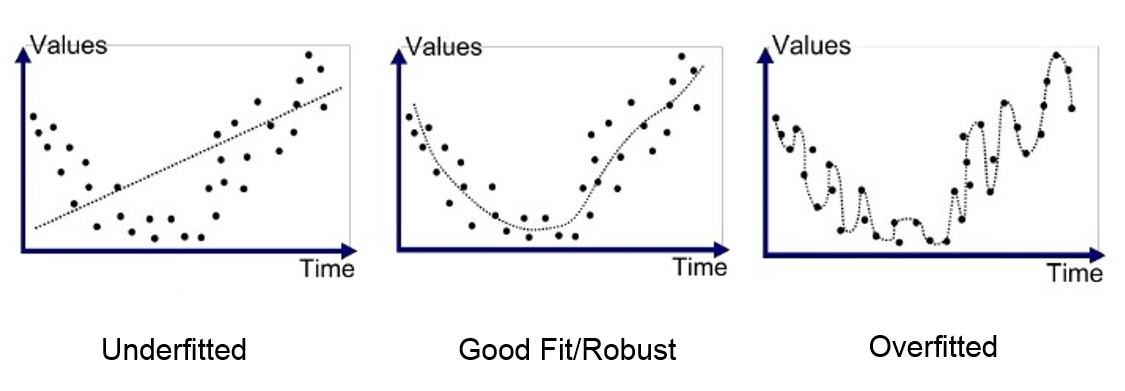
\includegraphics[width=.8\textwidth]{fitting}
		\caption{Illustratie van een underfitting, goeie fit en overfitting. Het eerste  model is duidelijk geen goed model omdat het niet aansluit bij de datapunten. het laatste model zal bij deze dataset een zeer goed model zijn, maar ook enkel voor dit model. Het is niet algemeen genoeg om op nieuwe data toe te passen. We proberen dus het middelste model te vinden die goed bij de punten aansluit maar niet te flexibel is.\cite{Bhande_2018}}
		\label{fig:fitting}
	\end{figure}
	
	Als een model te veel aangepast is aan de trainingsdata noemen we dit overfitting (rechts op figuur \ref{fig:fitting}), het model is dan te flexibel en probeert het model te dicht bij de trainingsdata te liggen. Het is belangrijk dat ons model algemeen is omdat we het model juist willen gebruiken om voorspellingen te doen op nieuwe data en niet op diezelfde trainingsdata, daarvan weten we namelijk al tot welke klasse ze behoren. Als ons model niet dicht genoeg bij de trainingsdata ligt noemen we dit underfitting (links op figuur \ref{fig:fitting}), het model is dan niet flexibel genoeg en er zal ook geen goeie voorspelling gemaakt worden op de validatiedata. We proberen dus de optimale metaparameters te bepalen (midden op figuur \ref{fig:fitting}).
	
\end{document}